\documentclass[11pt,]{article}
\usepackage{lmodern}
\usepackage{amssymb,amsmath}
\usepackage{ifxetex,ifluatex}
\usepackage{fixltx2e} % provides \textsubscript
\ifnum 0\ifxetex 1\fi\ifluatex 1\fi=0 % if pdftex
  \usepackage[T1]{fontenc}
  \usepackage[utf8]{inputenc}
\else % if luatex or xelatex
  \ifxetex
    \usepackage{mathspec}
    \usepackage{xltxtra,xunicode}
  \else
    \usepackage{fontspec}
  \fi
  \defaultfontfeatures{Mapping=tex-text,Scale=MatchLowercase}
  \newcommand{\euro}{€}
    \setmainfont{Georgia}
\fi
% use upquote if available, for straight quotes in verbatim environments
\IfFileExists{upquote.sty}{\usepackage{upquote}}{}
% use microtype if available
\IfFileExists{microtype.sty}{%
\usepackage{microtype}
\UseMicrotypeSet[protrusion]{basicmath} % disable protrusion for tt fonts
}{}
\usepackage[margin=1.0in]{geometry}
\ifxetex
  \usepackage[setpagesize=false, % page size defined by xetex
              unicode=false, % unicode breaks when used with xetex
              xetex]{hyperref}
\else
  \usepackage[unicode=true]{hyperref}
\fi
\hypersetup{breaklinks=true,
            bookmarks=true,
            pdfauthor={},
            pdftitle={},
            colorlinks=true,
            citecolor=blue,
            urlcolor=blue,
            linkcolor=magenta,
            pdfborder={0 0 0}}
\urlstyle{same}  % don't use monospace font for urls
\usepackage{graphicx,grffile}
\makeatletter
\def\maxwidth{\ifdim\Gin@nat@width>\linewidth\linewidth\else\Gin@nat@width\fi}
\def\maxheight{\ifdim\Gin@nat@height>\textheight\textheight\else\Gin@nat@height\fi}
\makeatother
% Scale images if necessary, so that they will not overflow the page
% margins by default, and it is still possible to overwrite the defaults
% using explicit options in \includegraphics[width, height, ...]{}
\setkeys{Gin}{width=\maxwidth,height=\maxheight,keepaspectratio}
\setlength{\parindent}{0pt}
\setlength{\parskip}{6pt plus 2pt minus 1pt}
\setlength{\emergencystretch}{3em}  % prevent overfull lines
\providecommand{\tightlist}{%
  \setlength{\itemsep}{0pt}\setlength{\parskip}{0pt}}
\setcounter{secnumdepth}{0}

%%% Use protect on footnotes to avoid problems with footnotes in titles
\let\rmarkdownfootnote\footnote%
\def\footnote{\protect\rmarkdownfootnote}

%%% Change title format to be more compact
\usepackage{titling}

% Create subtitle command for use in maketitle
\newcommand{\subtitle}[1]{
  \posttitle{
    \begin{center}\large#1\end{center}
    }
}

\setlength{\droptitle}{-2em}
  \title{}
  \pretitle{\vspace{\droptitle}}
  \posttitle{}
  \author{}
  \preauthor{}\postauthor{}
  \date{}
  \predate{}\postdate{}

\usepackage{booktabs}
\usepackage[final]{changes}
\usepackage[font={small},labelfont=bf,labelsep=colon]{caption}
\linespread{1.2}
\usepackage[compact]{titlesec}
\usepackage{enumitem}
\usepackage{tikz}
\def\checkmark{\tikz\fill[scale=0.4](0,.35) -- (.25,0) -- (1,.7) -- (.25,.15) -- cycle;}
\setlist{nolistsep}
\titlespacing{\section}{2pt}{*0}{*0}
\titlespacing{\subsection}{2pt}{*0}{*0}
\titlespacing{\subsubsection}{2pt}{*0}{*0}
\setlength{\parskip}{3pt}
\setremarkmarkup{(#2)}

% Redefines (sub)paragraphs to behave more like sections
\ifx\paragraph\undefined\else
\let\oldparagraph\paragraph
\renewcommand{\paragraph}[1]{\oldparagraph{#1}\mbox{}}
\fi
\ifx\subparagraph\undefined\else
\let\oldsubparagraph\subparagraph
\renewcommand{\subparagraph}[1]{\oldsubparagraph{#1}\mbox{}}
\fi

\begin{document}
\maketitle

\pagenumbering{gobble}

\section{Abstract}\label{abstract}

Alzheimers disease is terrible.

\clearpage

\section{Introduction}\label{introduction}

Something about AD\ldots{}

\section{Materials and Methods}\label{materials-and-methods}

\subsection{Imaging}\label{imaging}

\begin{table}[!htb]
  \centering
  \begin{tabular*}{1.0\textwidth}{@{\extracolsep{\fill}} rrrrr}
    \textbf{Subject id} & \textbf{Lesion count} & \textbf{Lesion load} & \textbf{Mean volume} & \textbf{[Min $-$ Max]} \\
    \toprule
    \midrule
    0 & 2 & 18 & 9 $\pm$ 1.4 & [8-10] \\
    1 & 3 & 3 & 1 $\pm$ 0 & [1-1] \\
    2 & 0 & 0 & 0 & [0-0] \\
    3 & 11 & 209 & 19 $\pm$ 18.4 & [1-56] \\
    4 & 3 & 130 & 43.3 $\pm$ 50.0 & [12-101] \\
    5 & 1 & 2 & 2 & [2-2] \\
    6 & 25 & 790 & 31.6 $\pm$ 29.2 & [2-132] \\
    7 & 24 & 767 & 32.0 $\pm$ 33.6 & [2-166] \\
    8 & 3 & 18 & 6 $\pm$ 7.8 & [1-15] \\
    9 & 21 & 508 & 24.2 $\pm$ 35.1 & [1-166] \\
    \midrule
    Total & 272 & 9191 & 33.8 $\pm$ 55.4 & [1-551] \\
    \midrule
    \bottomrule
  \end{tabular*}
\label{table:trainingData}
\caption{Sample table.
         }
\end{table}


An equation:

\[ F_1 =  \frac{ 2 \cdot TP }{ 2 \cdot TP + FP + FN}. \]

\begin{figure}[htbp]
\centering
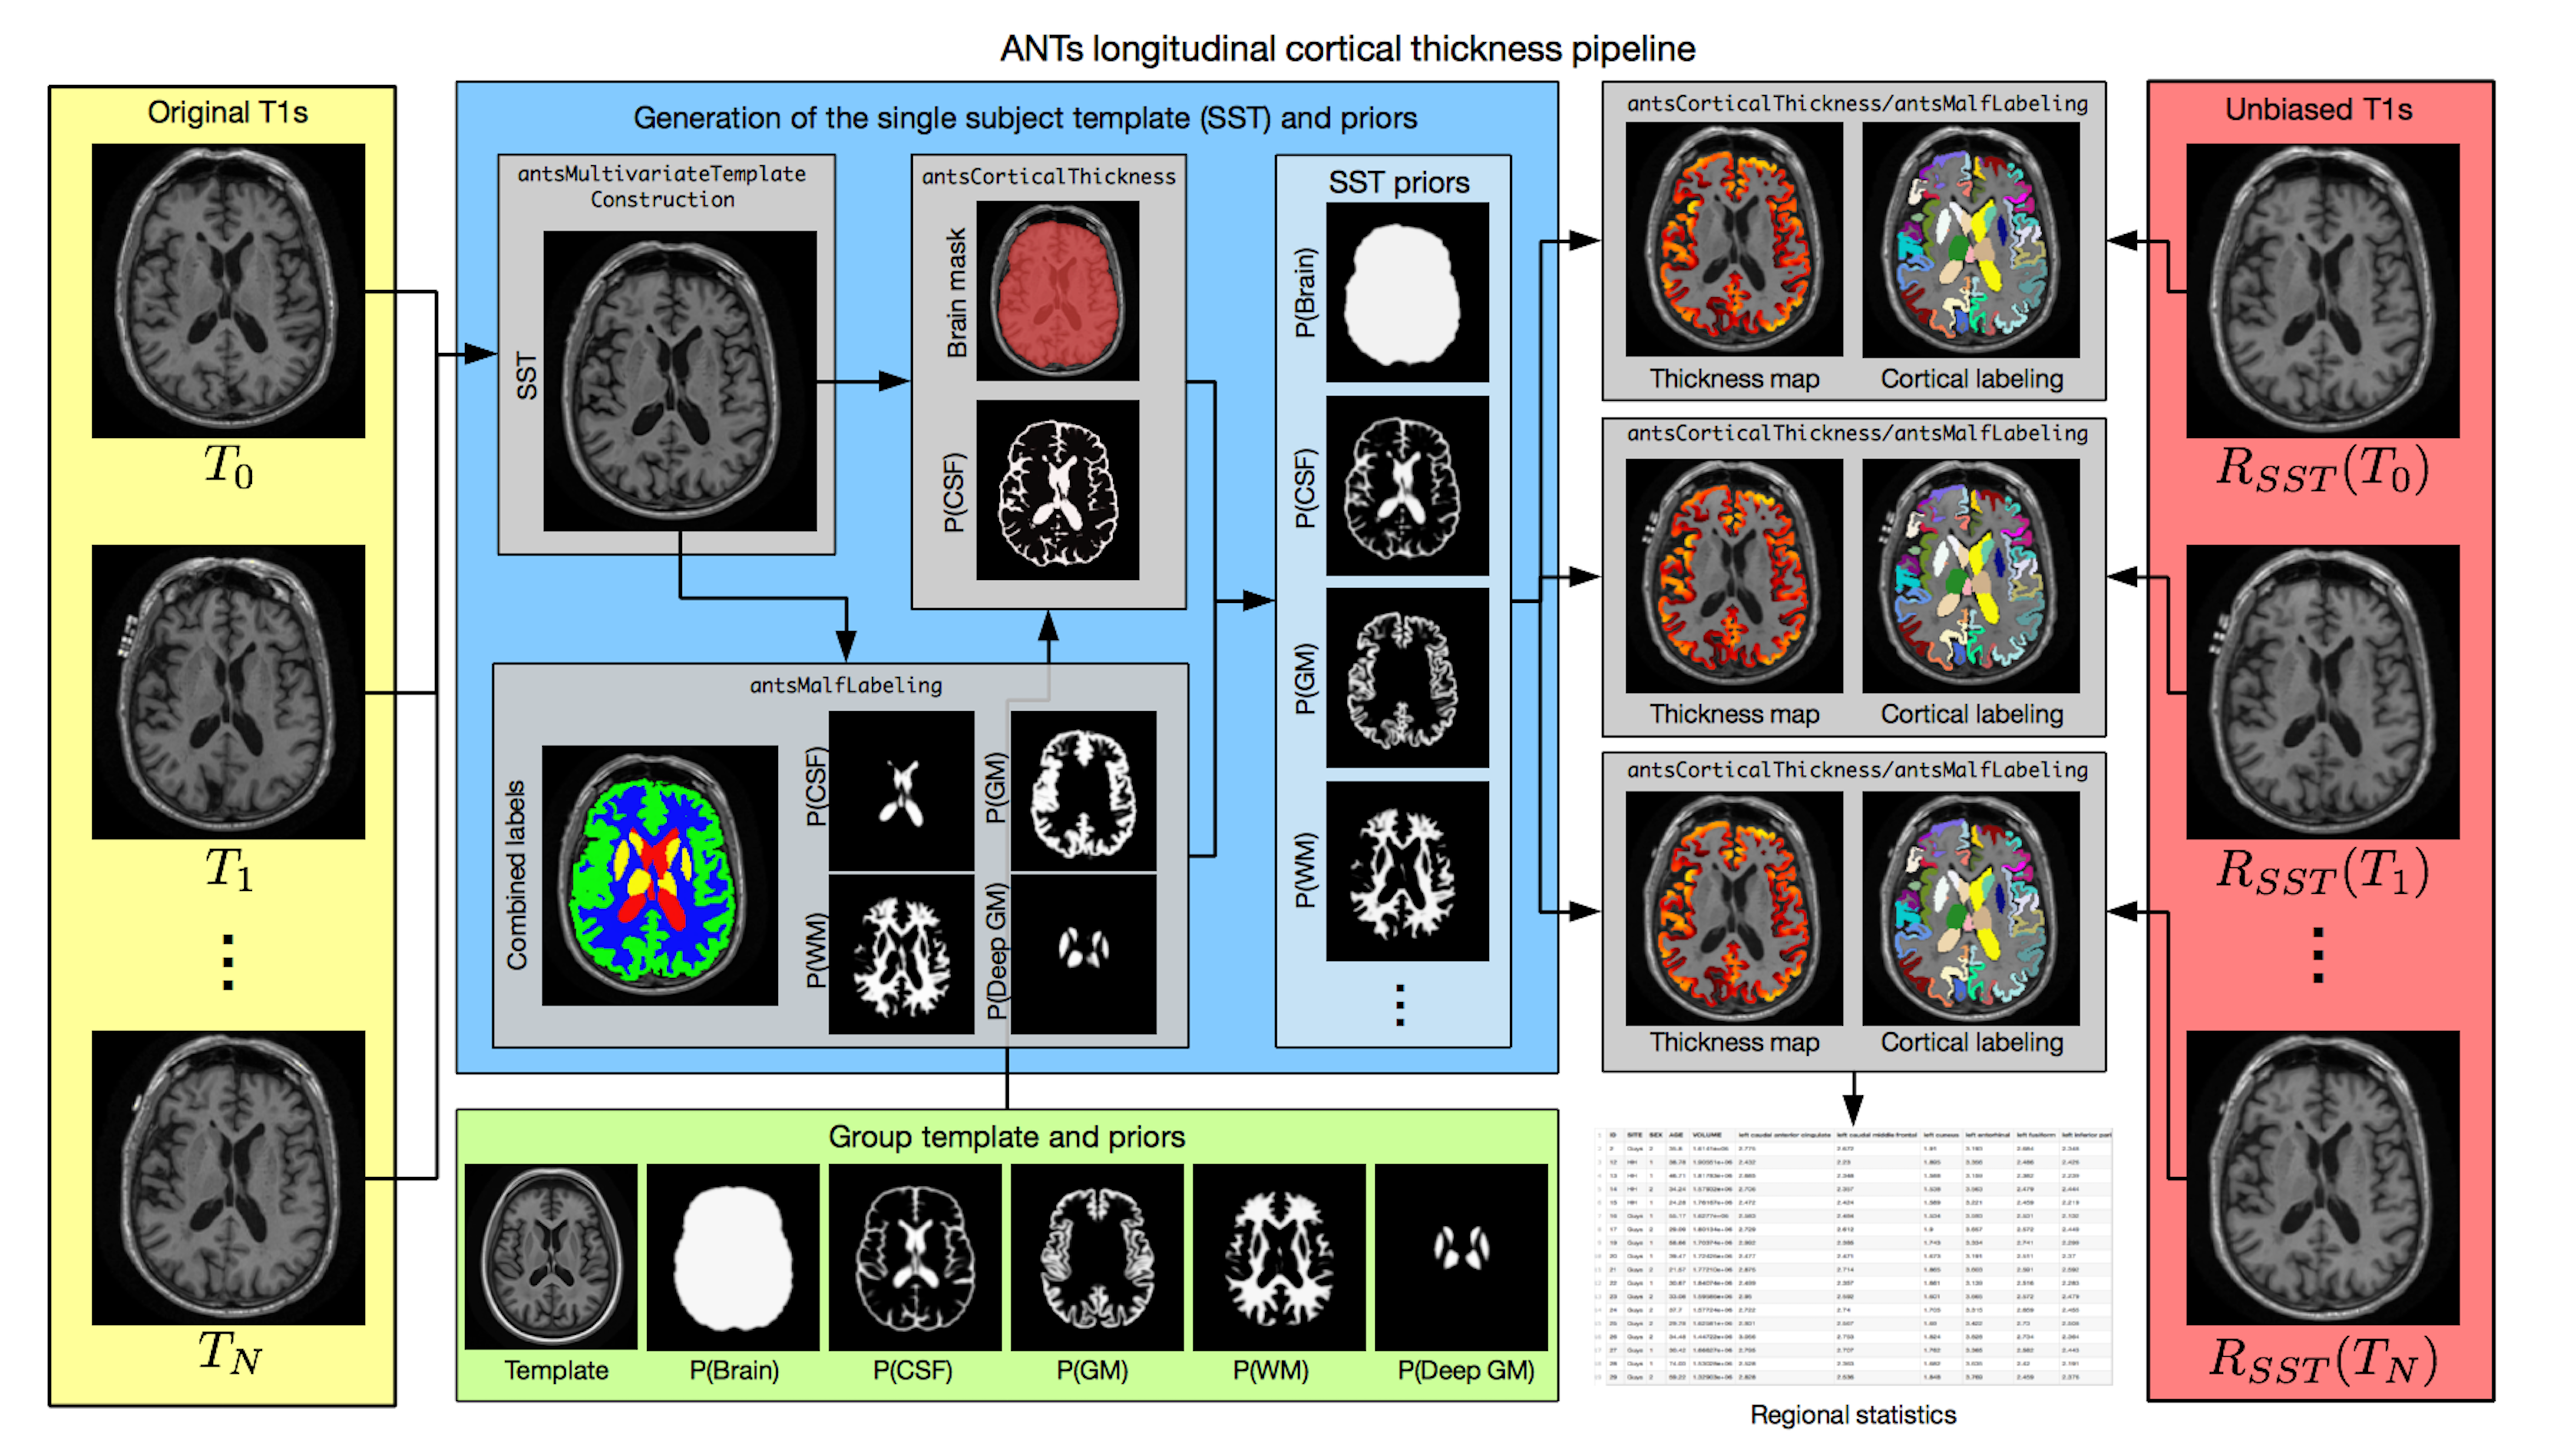
\includegraphics{../Figures/longitudinalPipeline.png}
\caption{Oh, and here is an image of the longitudinal pipeline with a
caption and a reference to the KellyKapowski paper {[}1{]}.}
\end{figure}

Here is an example footnote.\footnote{\textcolor{blue}{For comparison, the training data set of
  the MS Lesion Segmentation challenge
  associated with the international MICCAI 2008 conference has a mean lesion load of
  204 ($\pm$ 752) mm$^3$ per lesion and the resolution is almost twice what is used
  in this study (i.e., 0.5 $\times$ 0.5 $\times$ 0.5).}}

\section{Results}\label{results}

\section{Discussion}\label{discussion}

\subsection{Subsection 1}\label{subsection-1}

And a sweet equation:

\[ \exp^{-i \pi} = -1 \]

\clearpage

\hypertarget{refs}{}
\hypertarget{ref-Tustison:2014ab}{}
1. Tustison, N. J., Cook, P. A., Klein, A., Song, G., Das, S. R., Duda,
J. T., Kandel, B. M., Strien, N. van, Stone, J. R., Gee, J. C., and
Avants, B. B. ``\textbf{Large-Scale Evaluation of ANTs and FreeSurfer
Cortical Thickness Measurements}'' \emph{Neuroimage} 99, (2014):
166--79.
doi:\href{https://doi.org/10.1016/j.neuroimage.2014.05.044}{10.1016/j.neuroimage.2014.05.044}

\end{document}
